\chapter{アプローチ\label{sec:approach}}
\thispagestyle{plain}

本章では第\ref{sec:introduction}章で述べた問題に対する本研究のアプローチについて述べる.
第\ref{sec:introduction}章では以下の問題について述べた.

\begin{enumerate}[i.]
    \item 自身と近い作業嗜好を持つ人の募集を探すことが困難
    \item 参加の意思表明の心理的負担が大きい
\end{enumerate}

\section{自身と近い作業嗜好を持つ人の募集を探すことが困難\label{node:approach_i}}

本問題の原因の一つに作業通話の募集文に作業嗜好を判断する情報が少ないことが挙げられる.
特に開催時間や募集人数,開催場所などの情報が欠落していることが多い(図\ref{fig:tweet_recruitment}).
コミュニティ募集の場合,募集対象者は募集者の人柄や作業の進め方などは事前に把握していることが多いためこの問題は無視されることが多い.
一方,SNS募集の場合,募集者の人柄から自身の作業嗜好との相性を推察することができないため募集対象者の参加意欲を減衰させている可能性が高い.

この問題の解決には作業嗜好の可視化が効果的であるといえる.
作業通話の募集概要(募集対象者や開催時間など)を募集文に明示することで,募集対象者は参加するかの判断に必要な情報の多くを把握できる.
しかし,作業嗜好の要素として雰囲気の好みが挙げられるが,これについては募集概要から推察することは困難である.
作業通話における雰囲気(対話雰囲気)は参加者の気構えや心情が深く関わっており,作業の進め方や参加者の満足感に強く影響を与える要素である.
したがって,本研究では対話雰囲気が作業嗜好の大きな要素になると仮定し,対話雰囲気を推定し可視化するシステムの構築を行う.
また,本研究では対話雰囲気を「盛り上がり」,「真面目さ」など複数人からなる対話における場の空気感と定義する.

\begin{figure}
    \centering
    \fbox{
        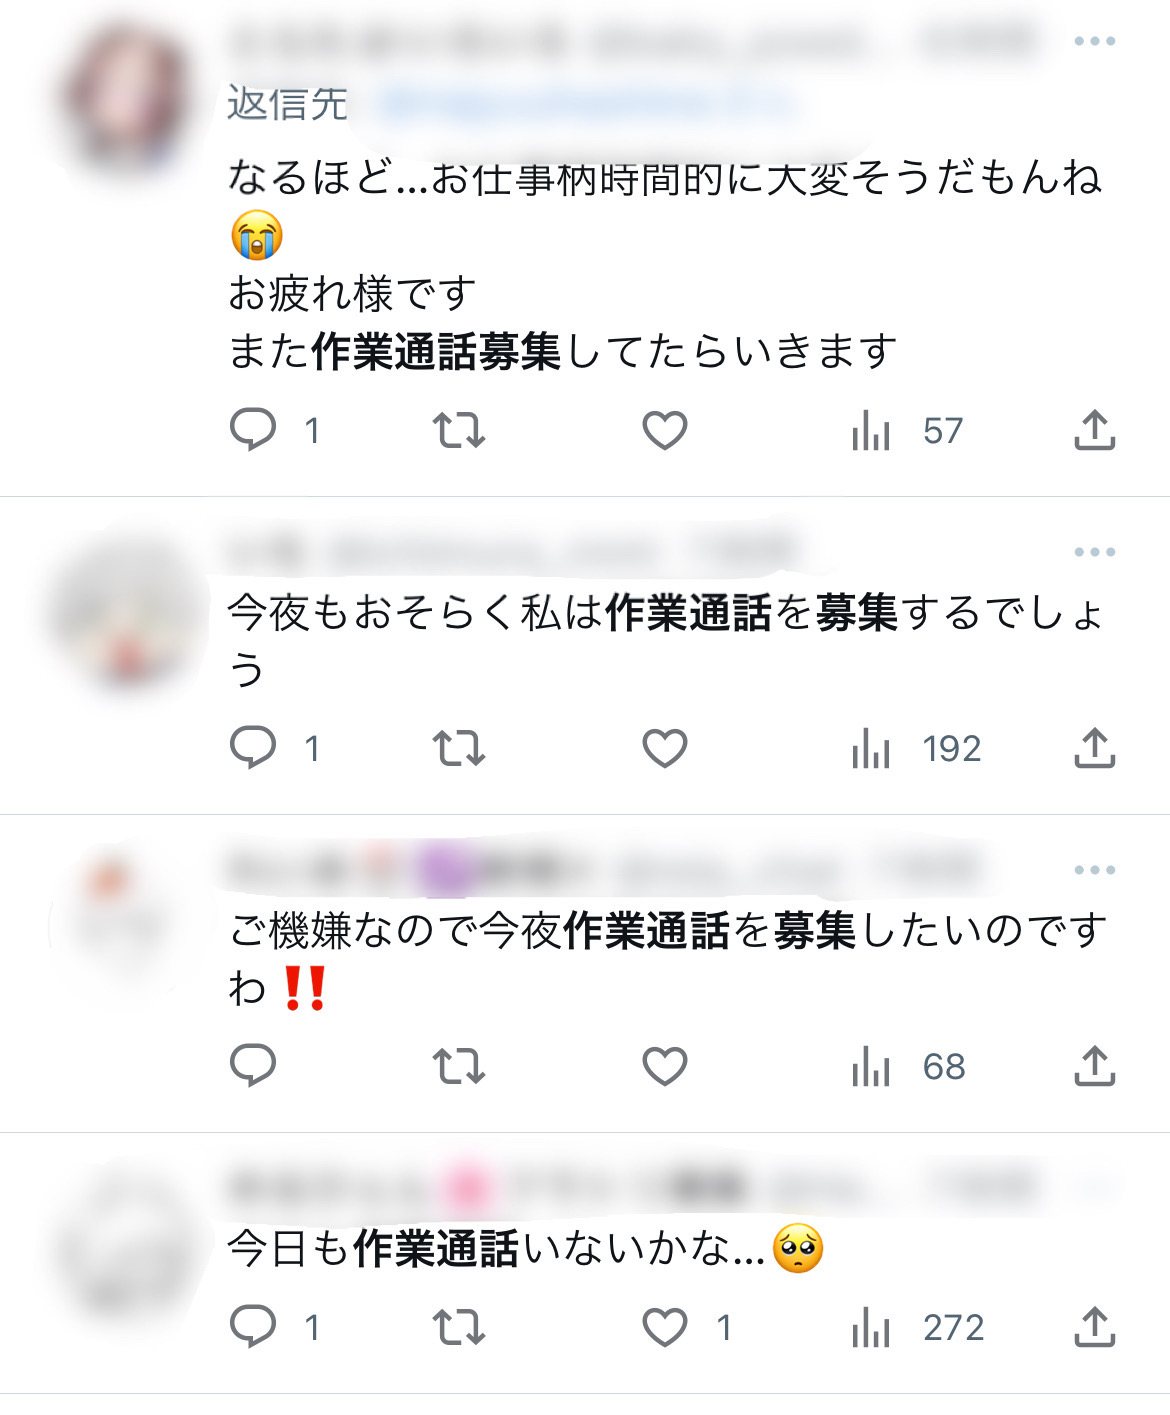
\includegraphics[width=0.7\textwidth]{figs/tweet_recruitment.jpg}
    }
    \caption{Twitterで「作業通話 募集」で検索した結果}
    \label{fig:tweet_recruitment}
\end{figure}

\section{参加の意思表明の心理的負担が大きい}

本問題の原因として,無縁ユーザとの作業通話という文化が十分に浸透していないことが挙げられる.
加えて,募集は募集以外の投稿と混在しながらフランクに投稿されている場合も多い.
また,第\ref{node:approach_i}節の問題も加わり募集文を見ただけではその募集がコミュニティ募集とSNS募集どちらなのかを判断することが難しいという問題もある.
これらのことから,募集対象者は興味のある募集を発見しても参加の意思表明をする心理的負担が大きいといえる.

そこで本研究では,第\ref{node:approach_i}節で述べたアプローチに加え,参加の意思表明の心理的負担の軽減を目的にSNS募集の枠組みを提案する.
具体的には,SNS募集における募集文(ツイート)を生成できるシステムの提案を行う.
またこのシステムは,SNS募集対象者が自身に向けて募集が行われていることや,そのような募集方法が存在することを明確に認知することで参加の意思表明の心理的負担の軽減を目指している.
このシステムは,システムを通したコミュニケーションは受け入れやすいということが報告されていることからも一定の効果が期待できる\cite{Harada}\cite{Kimura}\cite{Nishimura}\cite{Tsuzuki}.
このシステムを用いて作成された募集文には,第\ref{node:approach_i}節で述べた募集概要や対話雰囲気も併せて掲載することで,作業の透明性の向上を図りさらなる心理的負担の軽減を目指す.
